\documentclass[a4paper,11pt,dvipdfmx]{ujarticle}
% パッケージ
\usepackage{graphicx}
\usepackage{url}
% レイアウト指定を記述したファイルの読み込み
\input{layout}

% タイトルと氏名を変更せよ．
\title{日本におけるデジタル化の状況}
\author{G684872026 藤村　凛太郎}

\begin{document}

\maketitle %ここにタイトルが入る
\section{ブロードバンドの整備状況}
% ここから本文
% 節見出し: \section{}
% を使う
OECDによるブロードバンド回線の普及に関する調査\cite{oecd}によると、
図\ref{fig:21}に示すように,日本における100人あたりのモバイルブロードバンドの加入者数は190.5で,
第1位になっている。2位はエストニアで,３位米国と続く。
% 本文(1)
%  参考文献の参照: \cite{}
%  図番号の参照： \ref{}
% を使う
% 文献データベースのキーワードは oecd と imd
% になっている．
    %
    \begin{figure}[htbp]
    \centering
    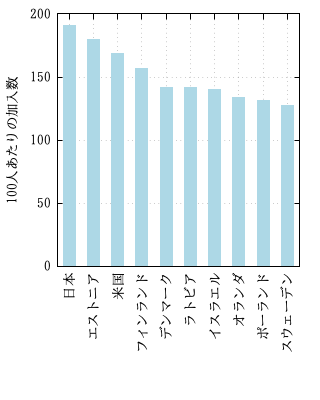
\includegraphics[width=0.6\linewidth]{fig21.png}
    \caption{ブロードバンドの整備状況}\label{fig:21}
\end{figure}

% 図の挿入
% \includegraphics{}
% を
% \begin{figure}[htbp]
% \end{figure}
% で囲み
% \caption{}
% で図のタイトルを入れる．
% \label{}
% を使って図番号が参照できるようにする
% また，
% \centering
% で図が中央に来るようにする

\section{デジタル競争力ランキング}

国際経営開発研究所（IMD）の調査\cite{imd}によると,
表\ref{tbl:デジタル競争力}に示すように,日本のデジタル競争力ランキングは調査対象の６４ヶ国中,
総合で28位,知識分野で25位となっている。
% ーーー
% 節見出し(2)
\begin{table}[htbp]
    \centering
    \caption{デジタル競争力ランキング（64か国中）}
    \label{tbl:デジタル競争力}

    \begin{tabular}{|l|c|c|}\hline
        国 & 総合 & 知識 \\
        \hline
        米国 & 1位 & 3位 \\
        \hline
        香港 & 2位 & 5位 \\
        \hline
        スウェーデン & 3位 & 2位 \\
        \hline
        デンマーク & 4位 & 8位 \\
        \hline
        シンガポール & 5位 & 4位 \\
        \hline
        韓国 & 12位 & 15位 \\
        \hline
        中国 & 15位 & 6位 \\
        \hline
        日本 & 28位 & 25位 \\
        \hline
    \end{tabular}
\end{table}
% 本文(2)

% 表の挿入
% \begin{tabular}
% \end{tabular}    
% による表の記述を 
% \begin{table}[htbp]
% \end{table}
% で囲み
% \caption{}
% で表のタイトルを入れる．
% \label{}
% を使って表番号が参照できるようにする
% また，
% \centering
% で表が中央に来るようにする

% ーーー
% 見出し(3)
% 考察
\section{考察}

\begin{itemize}
    \item 日本ではブロードバンド回線の普及率が高く，通信環境が整備されていることが分かった。
    \item しかし，デジタル競争力ランキングでは28位と，通信環境が良いだけで国際競争力は高くないことが分かった。
    \item そのため今後はIT人材の育成や、国内の技術開発を進めることが重要だと考えた。
\end{itemize}
%
% \begin{itemize}
% \end{itemize}
% を使って箇条書きで記述する

% ここに参考文献が入る
%
\bibliographystyle{junsrt}
\bibliography{exercise.bib}

\end{document}